\documentclass[10pt]{beamer}
\usetheme{metropolis}
\metroset{everytitleformat=regular}

\usepackage{booktabs}
\usepackage[scale=2]{ccicons}
\usepackage{pgfplots}
\usepackage{graphicx}
\usepackage{enumitem}
\usepackage{enumerate}

\usepackage{gensymb}

\usepackage{verbatim}

\usepackage{siunitx}

\usepgfplotslibrary{dateplot}
\graphicspath{{Images/}}
\usepackage{multirow}


\setbeamercolor{framesubtitle}{fg=mDarkTeal}
\addtobeamertemplate{frametitle}{}{%
  \ifx\insertframesubtitle\@empty\else%
  \usebeamerfont{framesubtitle}%
  \usebeamercolor[fg]{framesubtitle}%
  \insertframesubtitle%
  \fi%
}

\title{Saving Oneself}
\subtitle{Team One}
\date{May 4, 2016}
\author{John Boyer, Alexander Dwornik, Wojciech Dziwulski, Judah Rand}
\institute{University of Oxford}
\titlegraphic{\hfill
\includegraphics[height=1.3cm, width=4.23cm]{OxSlideLogo}}
\setbeamertemplate{bibliography item}{\insertbiblabel}
\begin{document}

\maketitle

\begin{frame}
  \frametitle{Table of Contents}
  \setbeamertemplate{section in toc}[sections numbered]
  \tableofcontents[hideallsubsections]
\end{frame}


\section{Chemical Preparation}
\begin{frame}{Overview \hspace{0pt plus 1 filll} \small{Alexander Dwornik}}

	\begin{itemize}[label={$\bullet$}]
		\item \textbf{Chemical Decomposition}
		\begin{itemize}[label={$\bullet$}]
			\item Decomposition of cells via autolysis and putrefaction causing significant damage to the sample
		\end{itemize}
		\item \textbf{Physical Deformation}
		\begin{itemize}[label={$\bullet$}]
			\item Due to the untreated brain being not rigid enough, damage would occur if sectioned untreated
		\end{itemize}
		\item \textbf{Poor Image Definition}
		\begin{itemize}[label={$\bullet$}]
			\item Due to the poor contrasting data, the images produced will not contain enough contrast to allow for synapse identification
		\end{itemize}
	\end{itemize}		
\end{frame}


\begin{frame}{Method Outline\hspace{0pt plus 1 filll} \small{Alexander Dwornik}}

\begin{itemize}
	\item [1.] Fixation and Cryopreservation
	\item [2.] Post-fixation and Staining
	\item [3.] Dehydration
	\item [4.] Embedding
\end{itemize}
\end{frame}

\begin{frame}{1. Fixation and Cryopreservation\hspace{0pt plus 1 filll} \small{Alexander Dwornik}}

\begin{columns}[T,onlytextwidth]
		\column{0.6\textwidth}
		\vspace{0.2cm}
		Method: \cite{McIntyre2015448}
\begin{itemize}
	\item [1.] Euthanasia
	\item [2.] Bilateral Carotid Cannulation
	\item [3.] Blood Washout Solution
	\item [4.] Perfusion of Fixative 
	\item [5.] Perfusion of Cryoprotectants
	\item [6.] Vitrification
	\item [7.] Brain Extraction
\end{itemize}	
Chemicals:
\begin{itemize}[label={$\bullet$}]
	\item 3\% w/v Glutaraldehyde Solution 
	\item 65\% w/v Ethylene Glycol 
\end{itemize}
		\column{0.4\textwidth}
		\begin{figure}
			\centering
			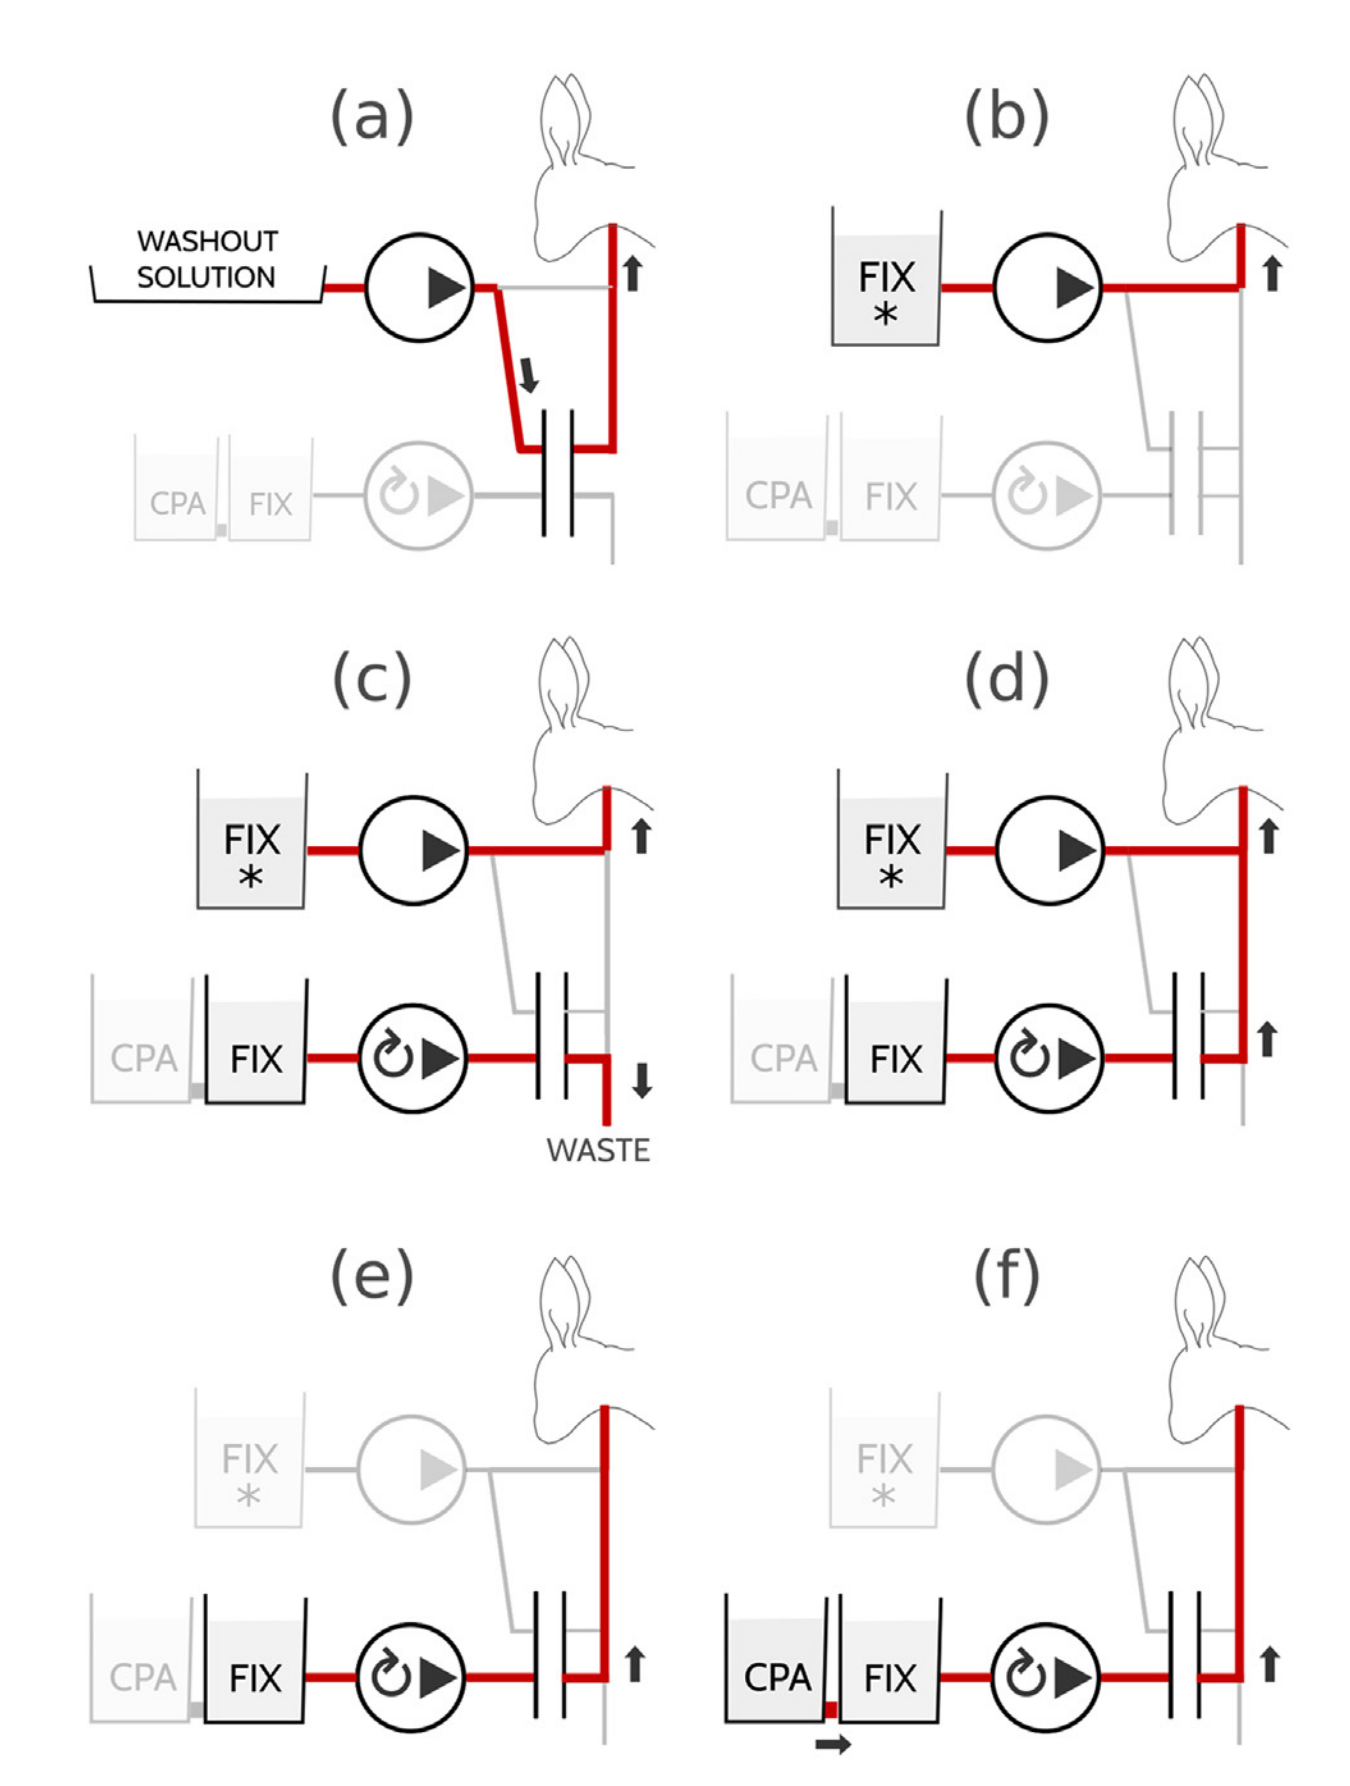
\includegraphics[totalheight=5cm,width=.3\paperwidth]{bunny_perfusion_diagram.png}
			\caption \small  Perfusion Transfer Method \cite{McIntyre2015448}
		\end{figure}
	\end{columns}
	
\end{frame}

\begin{frame}{2. Post Fixation and Staining\hspace{0pt plus 1 filll} \small{Alexander Dwornik}}

\begin{columns}[T,onlytextwidth]
		\column{0.6\textwidth}
		\vspace{0.2cm}
		\textbf{BROPA} \\
				Method: \cite{BROPA}
\begin{itemize}
	\item[1.] Initial Sectioning
	\item[2.] Intermediate Sectioning 
	\item[3.] Final Sectioning
	\item[4.] Removal of Cryoprotectants
	\item[5.] Diffusion of BROPA Chemicals
\end{itemize}	
Chemicals:
\begin{itemize}[label={$\bullet$}]
	\item Reduced Osmium and Formamide
	\item Osmium Tetroxide
	\item Pyrogallol
\end{itemize}
		\column{0.4\textwidth}
		\vspace{0.5cm}
		\begin{figure}
			\centering
			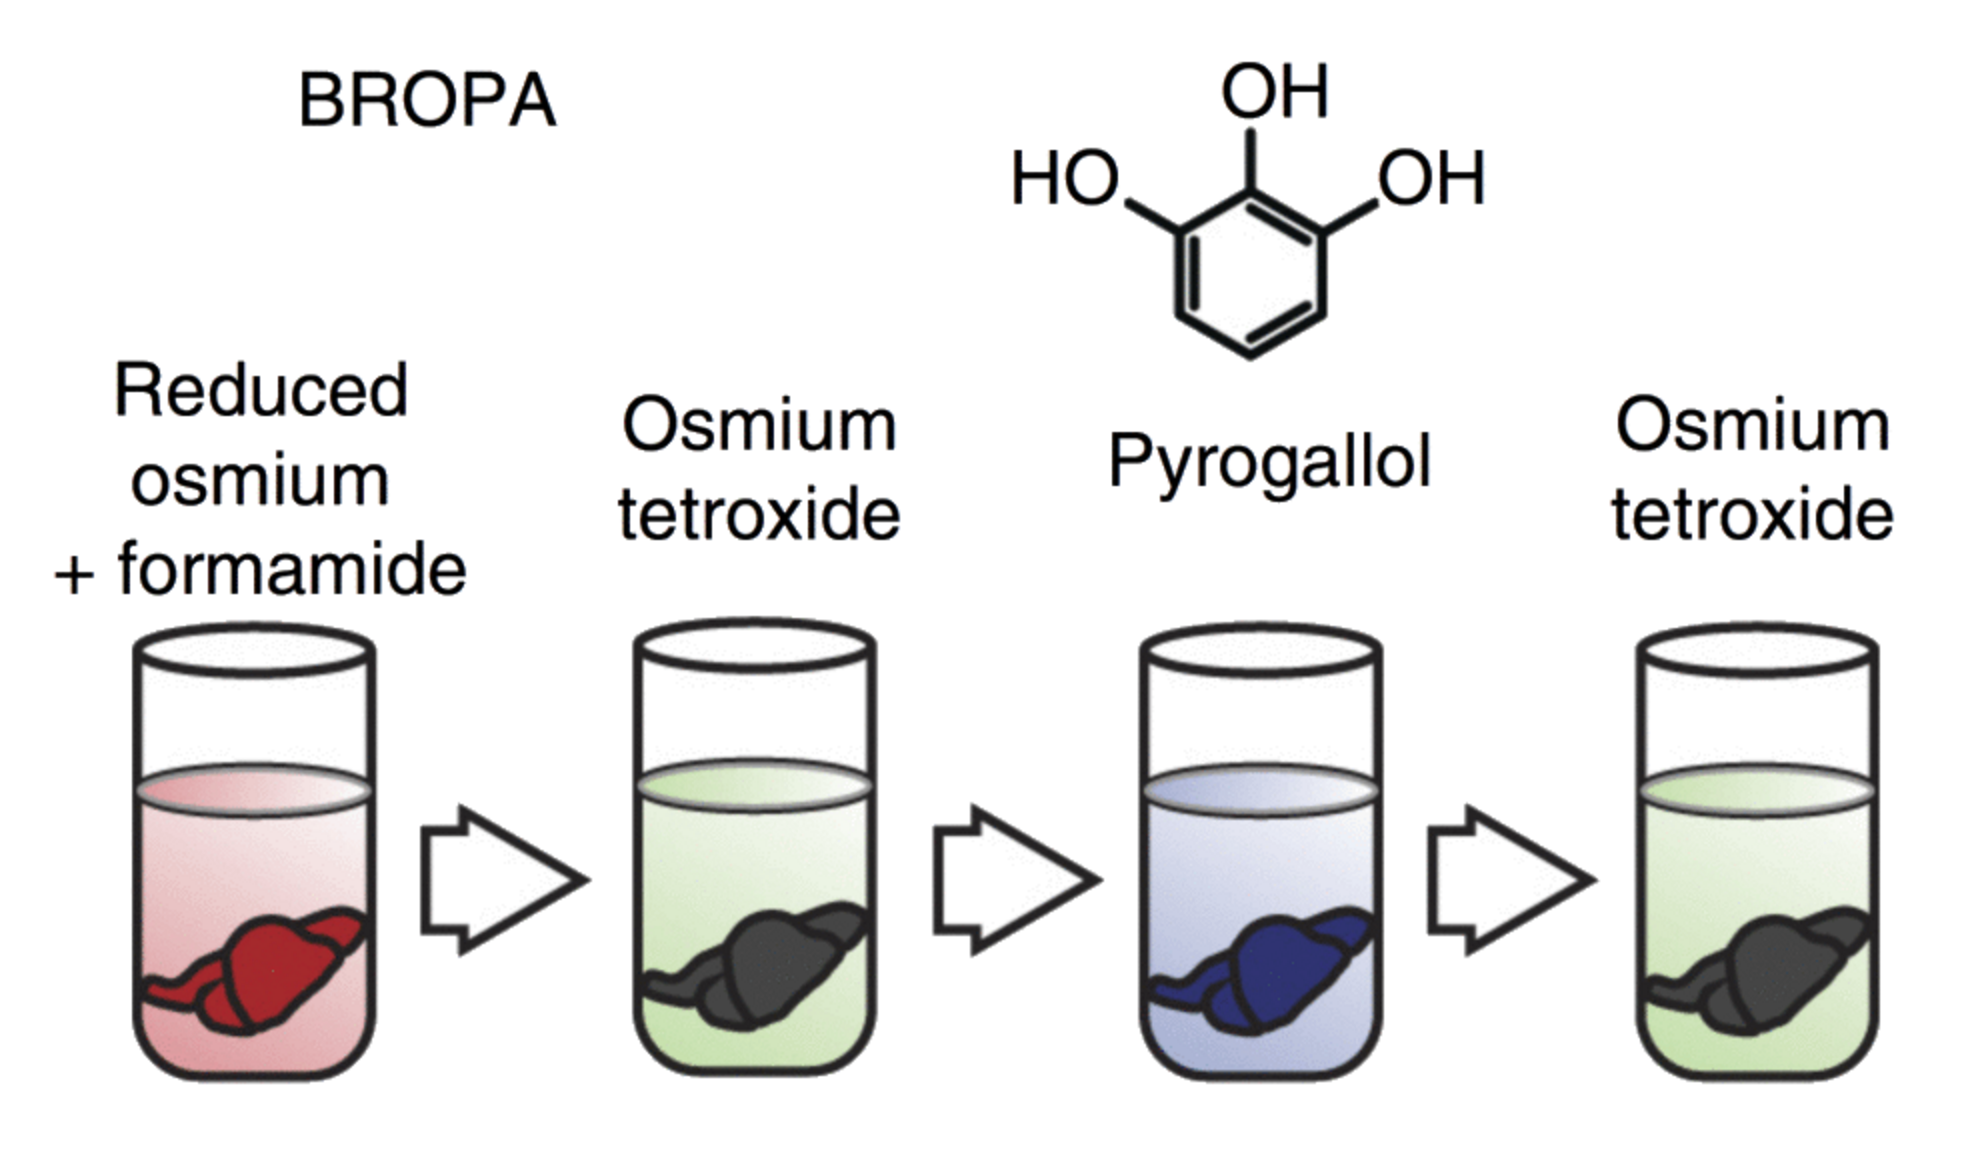
\includegraphics[totalheight=3cm,width=.3\paperwidth]{bropa.png}
			\caption \small  BROPA Method \cite{BROPA}
		\end{figure}
	\end{columns}
\end{frame}

\begin{frame}{3. Dehydration\hspace{0pt plus 1 filll} \small{Alexander Dwornik}}

\textbf{Solvent Dehydration} \\
				Method: \cite{dehydrationmethod}
				


\begin{itemize}
	\item[1.] Rinse sectioned sample for 20 minutes in double distilled water
	\item[2.] Transfer the sections of tissue into increasingly strong concentrations of ethanol
	\item[3.] Finish with a second 100\% ethanol solution for 1 hour
\end{itemize}	
	Chemicals:
\begin{itemize}[label={$\bullet$}]
	\item Ethanol
\end{itemize}
\end{frame}


\begin{frame}{4. Embedding\hspace{0pt plus 1 filll} \small{Alexander Dwornik}}


\textbf{Unicryl} \\
				Method: \cite{Unicryl}
				
\begin{itemize}
				 
\item[1.] Infiltrate with 100\% resin for 2 hours while agitating gently on a shaker or rotating wheel
\item[2.] Infiltrate with fresh resin for 10 hours to allow full penetration
\item[3.] Heat sample at 60\degree C for 48 hours
\end{itemize}
	
	\setlength\parindent{0pt}
	Chemicals: \\
	
\begin{itemize}[label={$\bullet$}]
	\item UNICRYL
\end{itemize}
\end{frame}

\begin{frame}{Automation and Cost\hspace{0pt plus 1 filll} \small{Alexander Dwornik}}

\begin{itemize}[label={$\bullet$}]
	\item By automating the chemical process, greater uniformity, efficiency and precision can be achieved
	\item By using 170 Lynx II for Microscopy machines, the process for chemically preparing the brain is completed in under a year
	\item Each Lynx II machines costs \textsterling13,750 \cite{lynxII} therefore the total cost for automation is  \textsterling2,454,375.00 (this cost includes maintenance) 
\end{itemize}
\end{frame}

\section{Method for Sectioning}
\begin{frame}{Overview \hspace{0pt plus 1 filll} \small{Judah Rand}}
	\begin{itemize}[label={$\bullet$}]
		\item \textbf{Inital Sectioning}
		\begin{itemize}[label={$\bullet$}]
			\item Reduce size of sections from complete brain without causing significant ultrastructure damage
		\end{itemize}
		\item \textbf{Intermediate Sectioning}
		\begin{itemize}[label={$\bullet$}]
			\item Further reduce size of sections to a size where final sectioning is possible
		\end{itemize}
		\item \textbf{Final Sectioning}
		\begin{itemize}[label={$\bullet$}]
			\item Sections must be thin enough to achieve sufficient Z-axis resolution
			\item Must have a practical sectioning speed
		\end{itemize}
	\end{itemize}		
\end{frame}

\begin{frame}{Initial Sectioning\hspace{0pt plus 1 filll} \small{Judah Rand}}
	\textbf{Precision Instruments VF-900 Compresstome}
	\begin{columns}[T,onlytextwidth]
		\column{0.7\textwidth}
		\vspace{1cm}
		\begin{itemize}[label={$\bullet$}]
			\item Brain embedded in agarose
			\item Sliced coronally with thickness \SI{0.5}{\milli\meter}
			\item Approximately 340 slices produced from a single brain
			\vspace{0.8cm}
			\item Only one machine required
			\item Quoted at \textsterling32,000 \cite{VF_900_price}
		\end{itemize}
		\column{0.3\textwidth}
		\begin{figure}
			\centering
			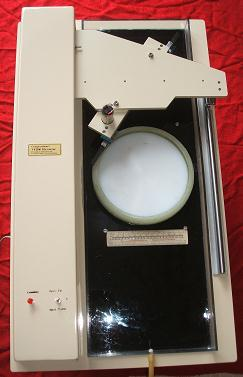
\includegraphics[totalheight=5cm,width=.3\paperwidth]{VF_900}
			\caption \small VF-900 Compresstome \cite{VF_900}
		\end{figure}
	\end{columns}
\end{frame}

\begin{frame}{Intermediate Sectioning\hspace{0pt plus 1 filll} \small{Judah Rand}}
	\textbf{Custom Vibratome}
	\begin{columns}[T,onlytextwidth]
		\column{0.5\textwidth}
		\vspace{0.5cm}
		\begin{itemize}[label={$\bullet$}]
			\item Coronal slices received from compresstome
			\item Slice divided up into blocks \SI{3.5}{\milli\meter} x \SI{2.5}{\milli\meter} x \SI{0.5}{\milli\meter}
			\item Approximately 1400 blocks per slice
			\item Approximately 6.3hrs per slice
			\vspace{0.8cm}
			\item Only one machine required
			\item Estimated cost \textsterling20,0000
		\end{itemize}
		\column{0.5\textwidth}
		\begin{figure}
			\centering
			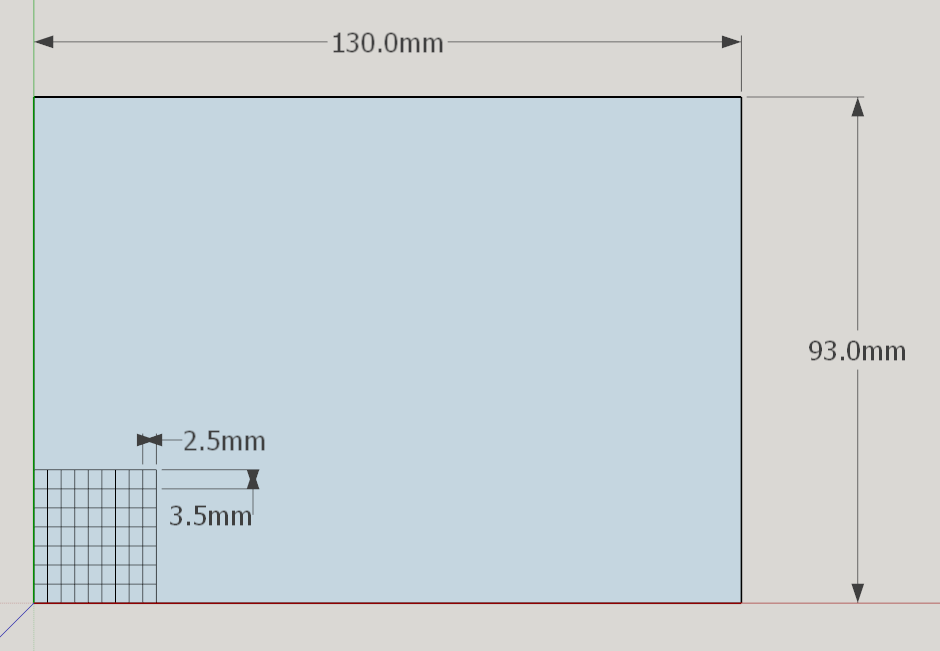
\includegraphics[width=.5\paperwidth]{brainslice}
			\caption \small Coronal brain slice modelled as a cuboid
		\end{figure}
	\end{columns}
\end{frame}

\begin{frame}{Intermediate Sectioning\hspace{0pt plus 1 filll} \small{Judah Rand}}
	\textbf{Custom Vibratome}
		\begin{figure}
			\centering
			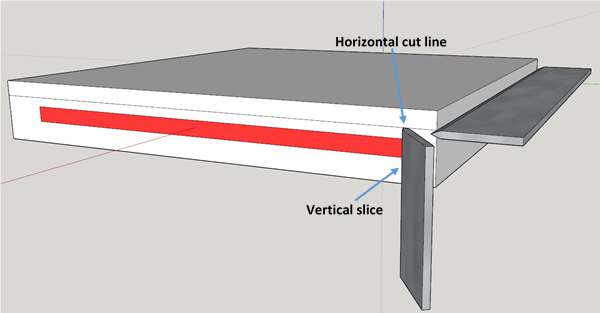
\includegraphics[width=.8\paperwidth]{custom_vibratome}
			\caption \small Design concept of custom vibratome
		\end{figure}
\end{frame}

\begin{frame}{Final Sectioning\hspace{0pt plus 1 filll} \small{Judah Rand}}
	\textbf{RMC Boeckeler ATUMtome}
	\begin{columns}[T,onlytextwidth]
		\column{0.7\textwidth}
		\begin{itemize}[label={$\bullet$}]
			\vspace{0.5cm}
			\item Developed in conjunction with the Lichtman Lab at Harvard
			\item Mount \SI{3.5}{\milli\meter} x \SI{2.5}{\milli\meter} x \SI{0.5}{\milli\meter} blocks
			\item $30nm$ thick sections
			\item Up to 10,000 sections per day possible \cite{hayworth2014atum}
			\vspace{0.5cm}
			\item One ATUMtome able to provide material for up to 40 microscopes
			\item 300 ATUMtomes are required, costing \textsterling50,000 each
		\end{itemize}
		\column{0.3\textwidth}
		\begin{figure}[label={$\bullet$}]
			\centering
			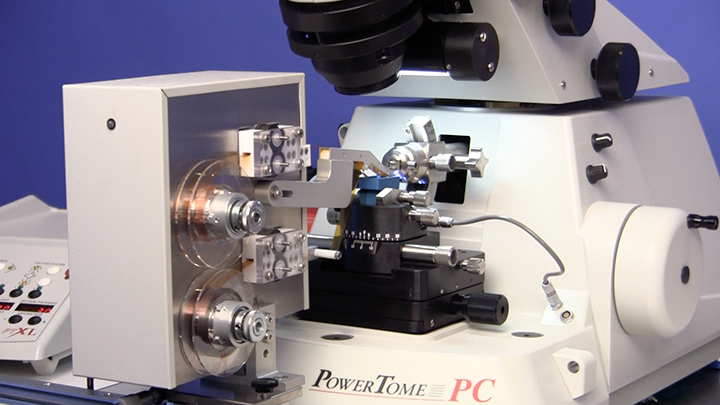
\includegraphics[totalheight=5cm,width=.3\paperwidth]{ATUMtome}
			\caption \small ATUMtome machine \cite{ATUMtome}
		\end{figure}
	\end{columns}
\end{frame}

\begin{frame}{Machine Costs\hspace{0pt plus 1 filll} \small{Judah Rand}}
	\begin{center}
		\begin{tabular}{|c|c|c|} 
			\hline
			\textbf{Machine}& \textbf{Number} & \textbf{Total Cost} \\ \hline
			VF-900 & 1 & \textsterling32,000 \\ \hline
			Custom Vibratome & 1 & \textsterling20,000 \\ \hline
			ATUMtome& 300& \textsterling15,000,000 \\ \hline
			\textbf{Total} & & \textsterling15,052,000 \\ \hline
		\end{tabular}
	\end{center}	
\end{frame}

\section{Recording Technology}

\begin{frame}{Silicon Wafers \hspace{0pt plus 1 filll} \small{John Boyer}}
	\textbf{Sectioning to Imaging Intermediary}
	\begin{columns}[T,onlytextwidth]
		\column{0.6\textwidth}
		\begin{itemize}[label={$\bullet$}]
			\vspace{1cm}
			\item Wafers received from the ATUMtome systems
			
			\item Each holds $\approx$ 5$\times$ $10^{-11} \text{m} ^3$ of brain tissue \cite{hayworth2014atum}
			
			\item Distributed among 12,000 microscopes
			
			\item Require approximately $4\times10^7$ uses
			\vspace{0.5cm}
			
			\item Will re-use around 120,000 
			\item Cost per wafer $\sim$ \pounds10 \cite{WaferPrice}
			
			
		\end{itemize}
		\column{0.4\textwidth}
		\begin{figure}
			\centering
			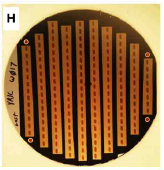
\includegraphics[totalheight=4cm,width=4cm]{silicon_wafer}
			\caption \small A 100mm silicon wafer with 162 ultrathin sections.\cite{hayworth2014atum}
		\end{figure}
	\end{columns}
\end{frame}



\begin{frame}{Linking \hspace{0pt plus 1 filll} \small{John Boyer}}
	\begin{itemize}[label={$\bullet$}]
		\item \textbf{Transport}
		\begin{itemize}[label={$\bullet$}]
			\item Wafers enter onto a conveyor system which is the beginning of the imaging pipeline
		\end{itemize}
		
		\item \textbf{Inital Imaging}
		\begin{itemize}[label={$\bullet$}]
			\item First the sections go through a very rapid light based imaging section (Around \pounds20,000 per light microscope e.g. the ZEISS Axio Imager A2 Vario \cite{ZeissAxio})
			\item No delays are introduced as the whole process is occurring in parallel with the second stage
			
		\end{itemize}
		
		\item \textbf{Loading}
		\begin{itemize}[label={$\bullet$}]
			\item The wafers are removed from the belt by a robotic arm 
			\item 12,000 robotic arms will be required, costing \pounds 10,000 per unit \cite{RoboArm}
		\end{itemize}
	\end{itemize}		
\end{frame}







\begin{frame}{Our Chosen Microscope \hspace{0pt plus 1 filll} \small{John Boyer}}
	\textbf{The MultiSEM 506}
	\begin{columns}[T,onlytextwidth]
		\column{0.6\textwidth}
		\begin{itemize}[label={$\bullet$}]
			
			
			\item Wafers are loaded into its vacuum chamber which automatically compresses
			
			\item Fiducial markers are identified via the ZEN software included\cite{ZeissLec}
			
			\item Automated imaging begins
			\item An area of approximately $2.55\times10^{-8}$m$^2$ is imaged in around 1.4s \cite{ZeissMulti}
			
			\vspace{0.5cm}
			\item Require around 12,000 machines for a 10 year imaging time
			\item Cost of \pounds 2.7 million per unit after speaking to Dr. Eberle at ZEISS
			
		\end{itemize}
		\column{0.4\textwidth}
		\begin{figure}
			\centering
			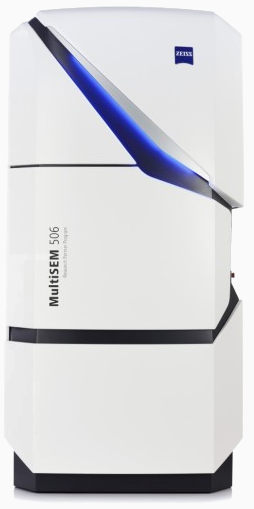
\includegraphics[totalheight=5cm,width=2.5cm]{multisem}
			\caption \small The MultiSEM 506 \cite{ZeissMulti}
		\end{figure}
	\end{columns}
\end{frame}


\begin{frame}{Machine Costs \hspace{0pt plus 1 filll} \small{John Boyer}}
	\begin{center}
		\begin{tabular}{|c|c|c|} 
			\hline
			
			\textbf{Machine}& \textbf{Number} & \textbf{Total Cost} \\ \hline
			Wafers& 120,000& \textsterling1,200,000\\ \hline
			Robo-Arm & 12,000 & \textsterling 120,000,000 \\ \hline
			Light Microscope & 12,000 & \textsterling240,000,000 \\ \hline
			MultiSEM& 12,000& \textsterling32,400,000,000\\ \hline
			
			\textbf{Total} & & \textsterling 32,761,200,000 \\ \hline
		\end{tabular}
	\end{center}	
\end{frame}



\section{Data and Software Challenges}

\begin{frame}[fragile]
  \frametitle{Data Organization  \hspace{0pt plus 1 filll} \small{Wojciech Dziwulski}}


 To decide on a standardisation model for storing our data two options were evaluated \\

  \begin{itemize}[label={$\bullet$}]
	  \item NeuroML - XML-based markup language storing metadata, membrane electrical properties and \textbf{anatomical structure and synaptic connectivity of neurons }
		  \cite{gleeson2010neuroml}
	  \item CAJAL3D with RAMON - Reusable Annotation Markup for Open coNnectomes - \textbf{lightweight} framework containing a set of minimum annotation data necessary for capturing the biological information 
	  		  \cite{kleissaslarge} 
  \end{itemize}
  
  \begin{center}
         Design choice - \alert{CALAJ3D with RAMON}\\
         $\downarrow$ \\
         Sufficiently robust, widely used, highly compressible
  \end{center}
  
  
  
\end{frame}

\begin{frame}[fragile]
  \frametitle{Data Querying  \hspace{0pt plus 1 filll} \small{Wojciech Dziwulski}}

  
  \metroset{block=fill}
  
    \begin{block}{WaferMapper (2014) }
		Image handling, mapping and alignment \cite{hayworth2014atum} 
    \end{block}

    \begin{block}{TrakEM2 (2012)}
        Computer-assisted identification and labelling of neurons \cite{cardona2012trakem2} 
    \end{block}
    
    \begin{block}{ConnectomeExplorer (2013)}
        Global statistical querying \cite{beyer2013connectomeexplorer} 
    \end{block}
    
    \begin{center}
             Design choice - \alert{USE THE THREE IN CONJUNCTION}\\
             $\downarrow$ \\
             Complimentary applications, open source
    \end{center}
  
\end{frame}

\begin{frame}[fragile]
  \frametitle{Data Storage  \hspace{0pt plus 1 filll} \small{Wojciech Dziwulski}}

  
\metroset{block=fill}

      \begin{block}{Image Storage - Requirements}
        Around \textbf{2M PB} (images) or \textbf{750 PB} (RAMON) for one human brain.
      \end{block}
     
      $ $
      
      \begin{columns}[T,onlytextwidth]
      	\column{0.5\textwidth}
      	\centering
      	$\downarrow$ \\
      	\alert{Local Storage}
      	
        \begin{itemize}[label={$\bullet$}]
        \item OCZ Vertex 4 SSD 512GB
        \item \pounds 100 $\times$ 1.5 million = \textbf{\pounds 150M}
        \item Simple and quick access
        \end{itemize}
      	
      	\column{0.5\textwidth}
      	\centering
      	$\downarrow$ \\
      	\alert{Cloud Storage}
      	
      	\begin{itemize}[label={$\bullet$}]
	    \item Amazon Glacier (AWS)
	    \item \pounds 0.005 / GB month $\times$ 10 years $\times$ 750PB  = \textbf{\pounds 190M}
	    \item Safe and gradually cheaper
        \end{itemize}
      	
      \end{columns}
      
      \begin{center}
      Use \textbf{Local Storage} - superior access speeds and price
      \end{center}
      
\end{frame}

\begin{frame}[fragile]
\frametitle{Segmentation  \hspace{0pt plus 1 filll} \small{Wojciech Dziwulski}}


\metroset{block=fill}
\begin{center}
\textbf{(1)} - Use VAST (manual) to produce \textbf{training data} \cite{kasthuri2015saturated} \\
$ $ \\
\textbf{(2)} - Use \textbf{machine learning} to segment automatically:
\end{center}
\begin{columns}[T,onlytextwidth]
	\column{0.25\textwidth}
	\centering
	Logistic regression
	\begin{figure}
			\centering
			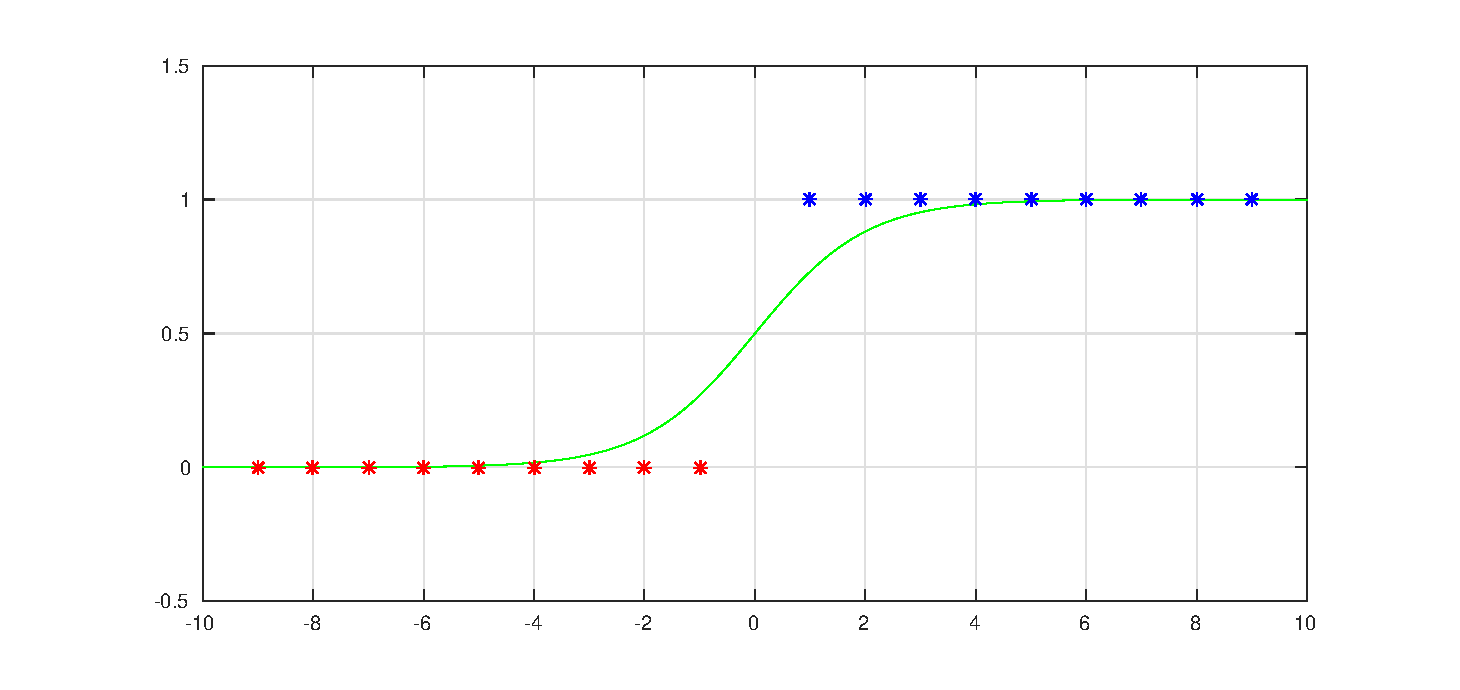
\includegraphics[width=.20\paperwidth]{logistic_regression.eps}
	\end{figure}
	\column{0.25\textwidth}
	\centering
	Random forests
	\begin{figure}
		\centering
		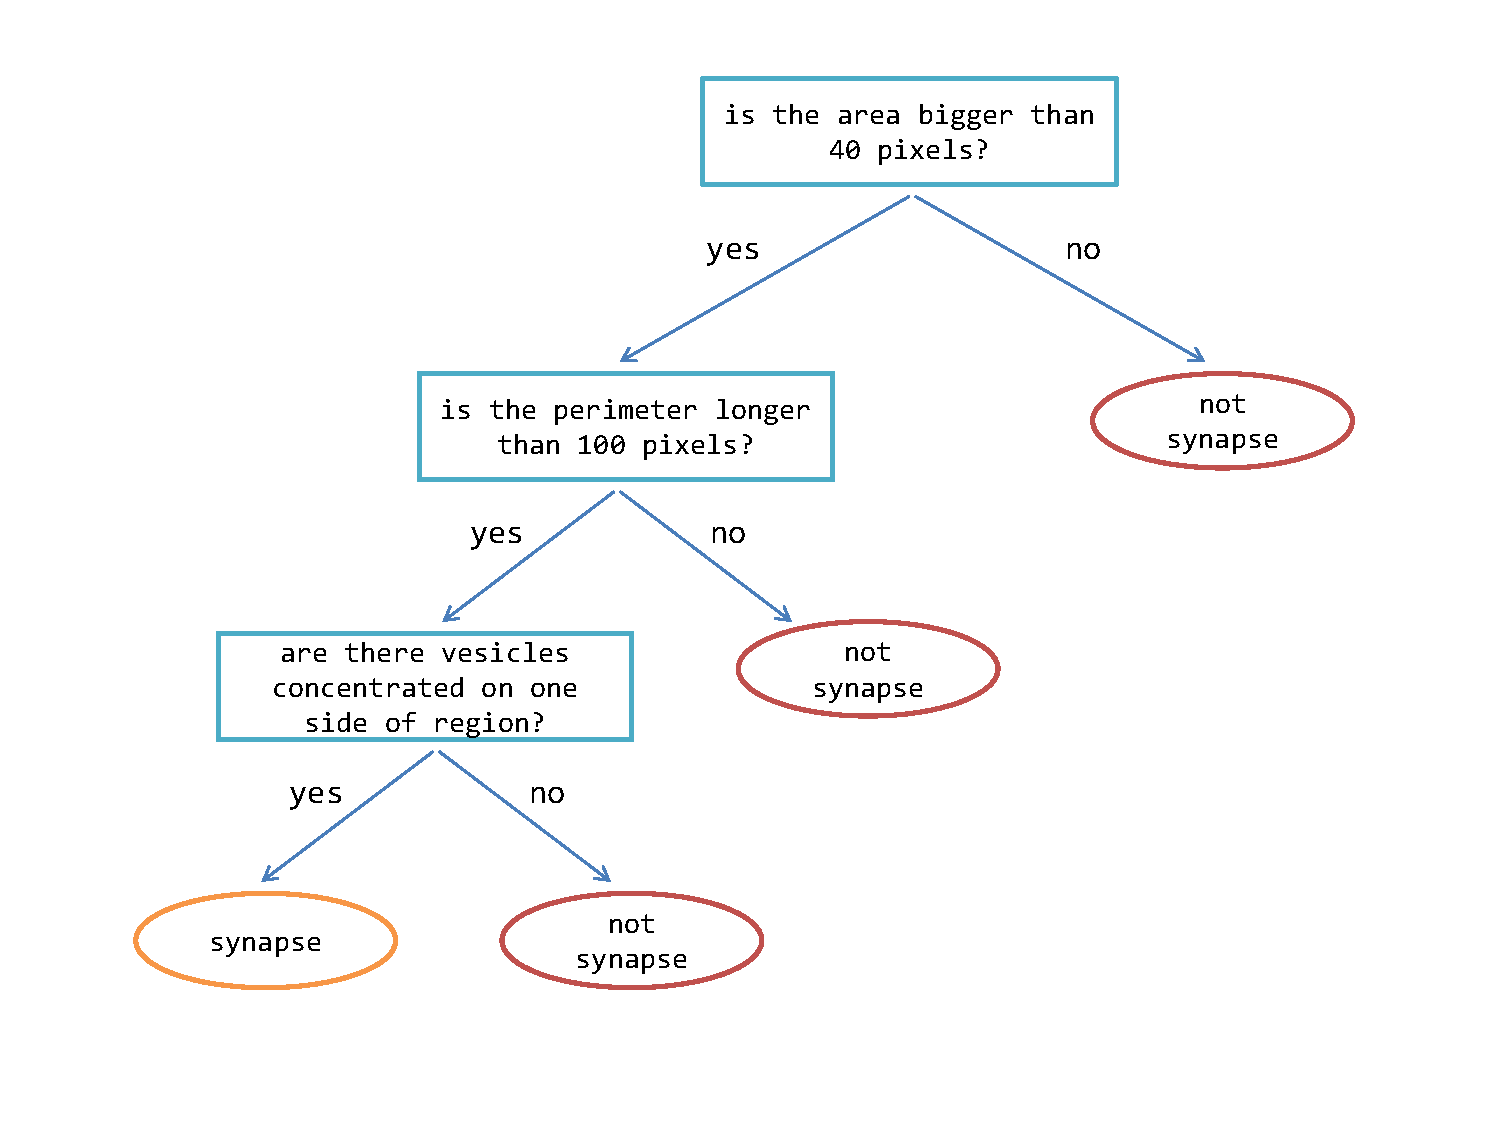
\includegraphics[width=.20\paperwidth]{decision_tree.pdf}
	\end{figure}
	\column{0.25\textwidth}
	\centering
	Neural networks
	\begin{figure}
		\centering
		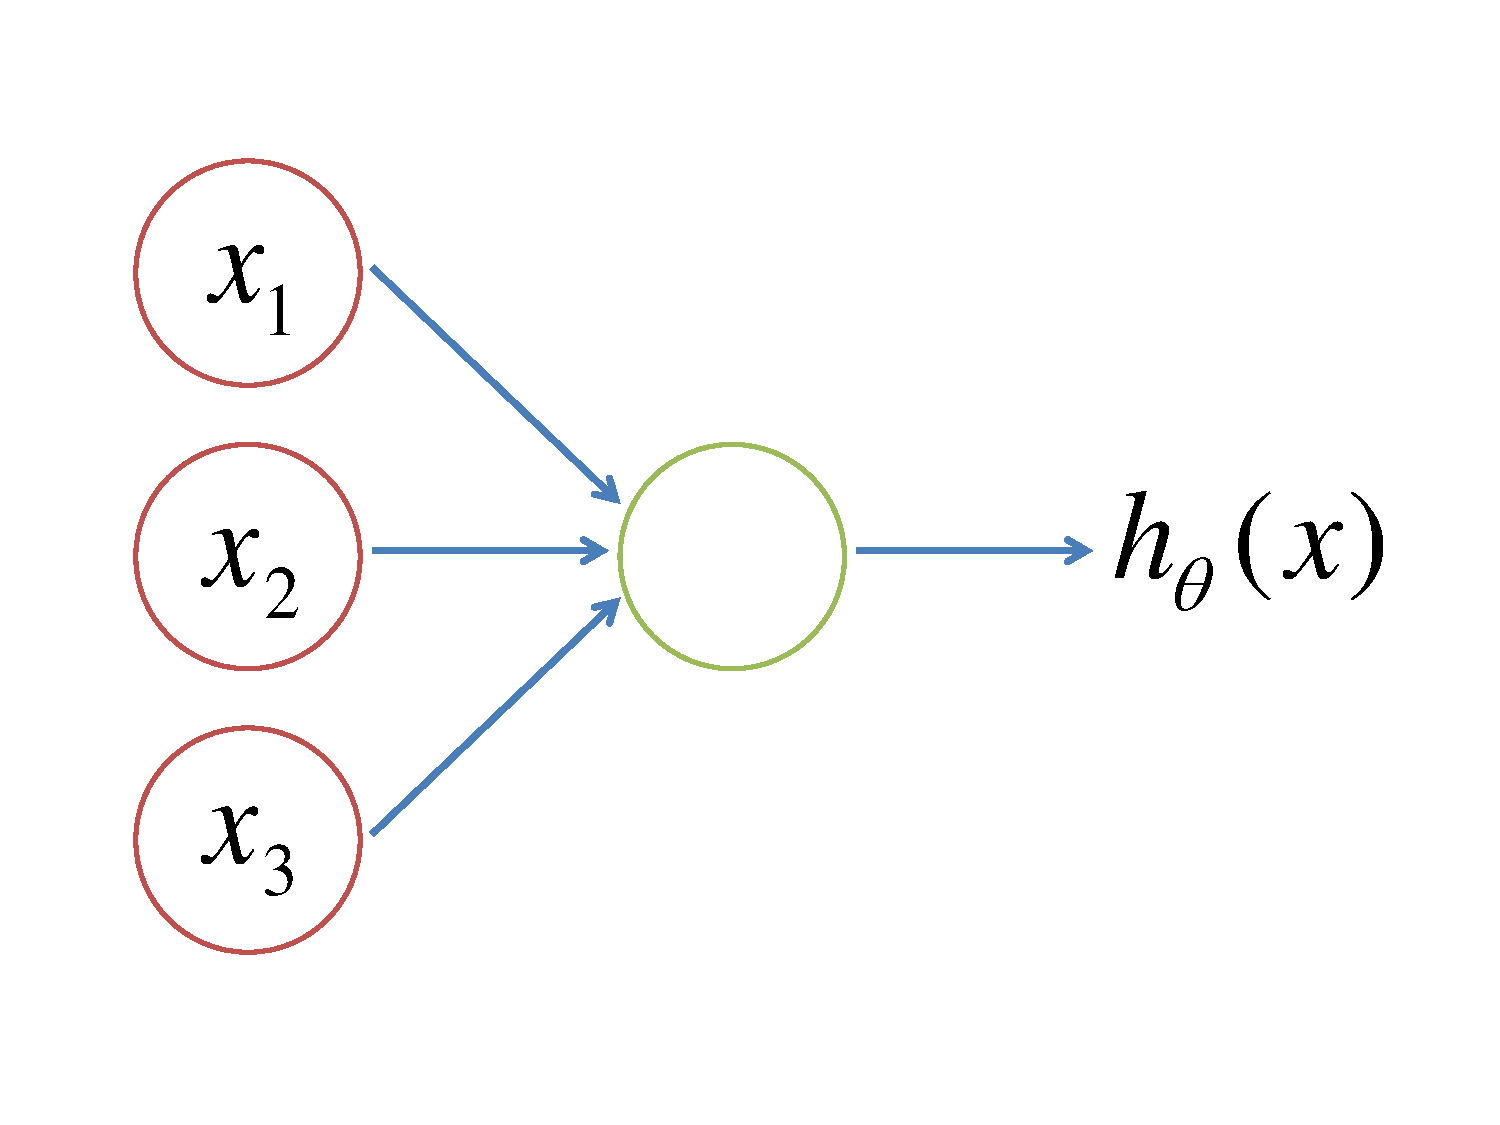
\includegraphics[width=.20\paperwidth]{logistic_unit.pdf}
	\end{figure}
	\column{0.25\textwidth}
	\centering
	Convolutional NN
	\begin{figure}
		\centering
		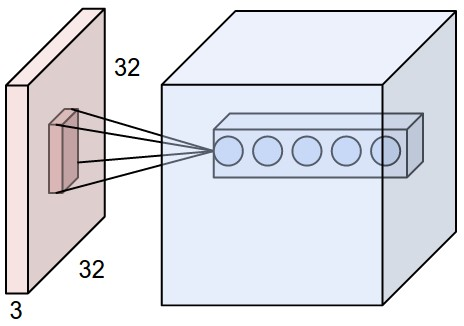
\includegraphics[width=.20\paperwidth]{depthcol.jpeg}
	\end{figure}
\end{columns}
  
\begin{center}
             After practical research - use \alert{RANDOM FORESTS}\\
             $\downarrow$ \\
             Along with the hand-designed features
\end{center}
  
\end{frame}

\begin{frame}[fragile]
  \frametitle{Feature Design  \hspace{0pt plus 1 filll} \small{Wojciech Dziwulski}}

  
  \metroset{block=fill}
  
  \begin{block}{Pixel by pixel}
  		Colour profiles, Gray scale statistics, Vesicle number and Concentration of \textbf{regions around all pixels}
  \end{block}

  \begin{block}{Regional}
      Preprocess the image to \textbf{generate false and true positives} \\ $\rightarrow$ Extract \textbf{geometrical features} (area, perimeter, etc.) (bottom figure)
  \end{block}
  
  (... then run the classifier on the above features) \\
  
  $ $ \\
  
  \alert{Regional Classification} - most successful (12.5\% accuracy)
  
  \begin{figure}
  			\centering
  			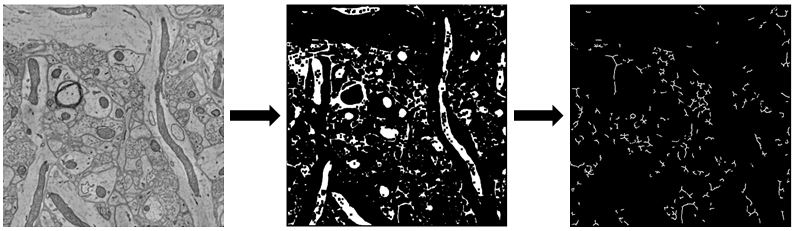
\includegraphics[width=.5\paperwidth]{pipeline.JPG}
  \end{figure}
\begin{center}

\end{center}

  
\end{frame}

\begin{frame}[fragile]
  \frametitle{Runtime and Hardware Requirements  \hspace{0pt plus 1 filll} \small{Wojciech Dziwulski}}

  
	\textbf{The need for speed:}
   		\begin{itemize}
   			\item \alert{(2009)} $3.2 \times 10^{10}$ years
   			\cite{mishchenko2009automation}
   			\item \alert{(2010)} $4.3 \times 10^9$ years
   			\cite{chklovskii2010semi}
   			\item for automatic reconstruction of a human brain
   		\end{itemize}
	      		
   10x increase every year $\Rightarrow$ \textbf{2 year segmentation in 2023} \\
   
   $ $ \\
   
   \textbf{Hardware} $\rightarrow$ NVIDIA Tesla K80 with CUDA platform \\
   \textbf{Cost} $\rightarrow$ 125,000 $\times$ \pounds 7000 = \pounds 875M
  
\end{frame}



\section{Conclusion}

\begin{frame}{Process Summary\hspace{0pt plus 1 filll} \small{John Boyer}}
	
	\begin{itemize}[label={$\bullet$}]
		\item First class amenities in Belgium
		\item Preliminary procedures for surgery and preservation
		\item Full brain cryo-storage
		\item Sectioning
		\item Imaging
		\item Synapse identification and Storage
		\item Future reanimation
	\end{itemize}
	
\end{frame}

\begin{frame}{Cost Summary\hspace{0pt plus 1 filll} \small{John Boyer}}
	
	\begin{table}
		
		
		\begin{tabular}{|c|c|} 
			\hline
			\textbf{Pipeline}&  \textbf{Approximate Total Cost} \\ \hline
			Chemical &\textsterling 0.004 Billion \\ \hline
			Sectioning &\textsterling 0.098 Billion \\ \hline
			Imaging &\textsterling 33.031 Billion  \\ \hline
			Data & \textsterling 1.705 Billion  \\ \hline
			Contingency/Misc & \textsterling 5.000 Billion  \\ \hline
			\textbf{Total} & \textsterling 39.840 Billion \\ \hline
		\end{tabular}
	\end{table}
	
	\begin{itemize}[label={$\bullet$}]
		\item The cost for scanning the first brain is \pounds 5 Billion
		\item Will receive income from multiple interested sources, including human preservation societies, research grants and a secondary business of brain storage
	\end{itemize}
	
\end{frame}

\plain{Questions?}

\begin{frame}[allowframebreaks]

  \frametitle{References}

  \bibliography{bib}
  \bibliographystyle{abbrv}

\end{frame}

\end{document}
